% ------------------------------------------------------------------
%  Figura: Hotspot Spoofing — 4 pasos (slide 19)
%  Diseño compacto horizontal con iconos de color
% ------------------------------------------------------------------
\documentclass[border=0.2cm]{standalone}
\usepackage[utf8]{inputenc}
\usepackage[T1]{fontenc}
\usepackage{libertine}
\usepackage{tikz}
\usepackage{xcolor}

\definecolor{primary}{HTML}{280091}
\definecolor{secondary}{HTML}{4C5CC5}
\definecolor{accent}{HTML}{3FCFD5}
\definecolor{exgreen}{HTML}{00B299}
\definecolor{alertred}{HTML}{C0392B}
\definecolor{darkgray}{RGB}{80,80,80}

\begin{document}
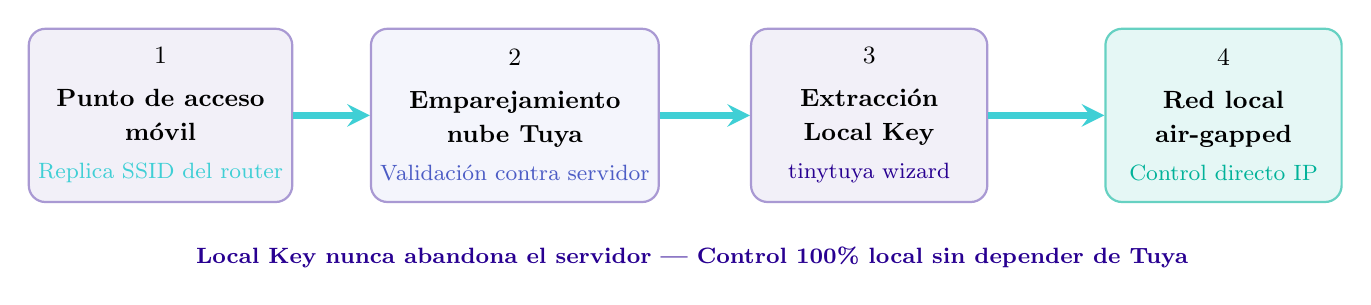
\begin{tikzpicture}[
  box/.style={draw=primary!40, fill=white, rounded corners=6pt,
              minimum width=3cm, minimum height=2.2cm, align=center,
              font=\small, line width=0.8pt},
  num/.style={font=\Large\bfseries\color{primary}},
  conn/.style={draw=accent, line width=2.5pt, ->, >=stealth, rounded corners=2pt},
]

\node[box, fill=primary!6] (s1) at (0, 0) {
  {\num 1}\\[0.15cm]
  \textbf{Punto de acceso}\\[0.05cm]
  \textbf{móvil}\\[0.1cm]
  {\footnotesize\color{accent}Replica SSID del router}
};

\node[box, fill=secondary!6] (s2) at (4.5, 0) {
  {\num 2}\\[0.15cm]
  \textbf{Emparejamiento}\\[0.05cm]
  \textbf{nube Tuya}\\[0.1cm]
  {\footnotesize\color{secondary}Validación contra servidor}
};

\node[box, fill=primary!6] (s3) at (9, 0) {
  {\num 3}\\[0.15cm]
  \textbf{Extracción}\\[0.05cm]
  \textbf{Local Key}\\[0.1cm]
  {\footnotesize\color{primary}tinytuya wizard}
};

\node[box, fill=exgreen!10, draw=exgreen!60] (s4) at (13.5, 0) {
  {\num 4}\\[0.15cm]
  \textbf{Red local}\\[0.05cm]
  \textbf{air-gapped}\\[0.1cm]
  {\footnotesize\color{exgreen}Control directo IP}
};

\draw[conn] (s1.east) -- (s2.west);
\draw[conn] (s2.east) -- (s3.west);
\draw[conn] (s3.east) -- (s4.west);

\node[font=\footnotesize\bfseries\color{primary}] at (6.75, -1.8) {
  Local Key nunca abandona el servidor — Control 100\% local sin depender de Tuya
};

\end{tikzpicture}
\end{document}
